\documentclass[12pt]{article} % Sets normal text font size to 12pt
\usepackage[hidelinks,linktoc=all]{hyperref}
\usepackage{sectsty} % Ermöglicht Anpassung der Schriftarten für Überschriften
\usepackage[a4paper, margin=2.5cm]{geometry}
\usepackage{xcolor}
\usepackage{soul}
\usepackage{graphicx}
\usepackage{float}
\usepackage{subcaption}
\usepackage{siunitx}
\usepackage{listings}
\usepackage{xcolor}

\lstdefinestyle{pythonwide}{
    language=Python,
    basicstyle=\ttfamily\footnotesize,
    keywordstyle=\color{blue},
    commentstyle=\color{gray},
    stringstyle=\color{red},
    showstringspaces=false,
    breaklines=true,
    breakatwhitespace=false,
    columns=fullflexible,
    keepspaces=true,
    frame=single,
    captionpos=b,
    xleftmargin=0.01\textwidth,
    xrightmargin=0.01\textwidth,
    framexleftmargin=0.01\textwidth,
    numbers=none
}

\title{\textbf{\fontsize{50}{60}\selectfont TU München}\\ % Make "TU München" bold
\vspace{0.5cm} \textbf{\Huge Bericht der Ingenieurspraxis} \\ % Make "Bericht der Ingenieurspraxis" bold
\vspace{0.3cm} \Large B.Sc. Elektrotechnik und Informationstechnik} % Keep "B.Sc. ..." normal

\date{} % Remove the default date

\sectionfont{\Large} % Adjusts section font size
\subsectionfont{\large} % Adjusts subsection font size

\renewcommand{\contentsname}{Inhaltsverzeichnis} % Change the title of the table of contents

\begin{document}

\maketitle

\vspace{2cm} % Add space after the main title

% Additional information
\begin{center}
    \Large \textit {Betreuender Professor:} \\ Prof. Dr.-Ing. Thomas Eibert \\[0.5cm]
    \Large \textit {Fachgebiet:} \\ Lehrstuhl für Hochfrequenztechnik \\[0.5cm]
    \Large \textit {Student:} \\ Marcelo Leindl\hspace{0.5cm}03787928
\end{center}

\newpage

% Inhaltsverzeichnis
\tableofcontents
\newpage

\section{Praktikumsstelle I: Comet AG}

\subsection{Ausgangslage und Aufgabenstellung}
Nach der Einführung von neuen Produkten im X-Ray Lineup von Comet werden neue Test-Pipelines benötigt, welche auf Stabilität, technischer Korrektheit und Einhalten von Boundaries prüfen.
Produkte, die bereits ausgeliefert werden, sind schon in einem täglichen Testprotokoll enthalten, in dieser müssen die neuen Produkte integriert werden.
Die existierenden Tests müssen nach dem Don't repeat yourself Prinzip (DRY) überarbeitet werden und wenn möglich generisch gestaltet werden, damit sie für die einzelnen Produkte wiederverwendbar sind.

\subsection{Unternehmen, Produkte und technischer Hintergrund}

\subsubsection{Einordnung der Abteilung und der bearbeiteten Produkte}
Die Ingenieurspraxis wurde in der Industrial X-Ray Modules (IXM) Abteilung von Comet AG durchgeführt. Von der größeren Produktauswahl der Division hat sich mein Arbeitsaufwand wesentlich auf die folgenden drei spezialisiert.
\\
\\
\textbf{Xplorer Series} (micro focus) ist ein Röntgenmodul für hochauflösende Inline-Inspektionen kleiner Bauteile in industriellen Produktionsprozessen. Typischer Anwendungsfall ist die Qualitätskontrolle von Halbleiterbauteilen und Lithium-Ionen-Batteriezellen auf kleinste Defekte.
Der Xplorer 130 arbeitet mit einer maximalen Röhrenspannung von 130 kV und erreicht eine minimale Auflösung von 5 µm. Die maximale Leistung beträgt 30 W mit einer Strahlungsabdeckung von 115° in beiden Achsen.
\\
\\
\begin{figure}[H]
    \centering
    
    \begin{subfigure}{0.40\textwidth}
        \centering
        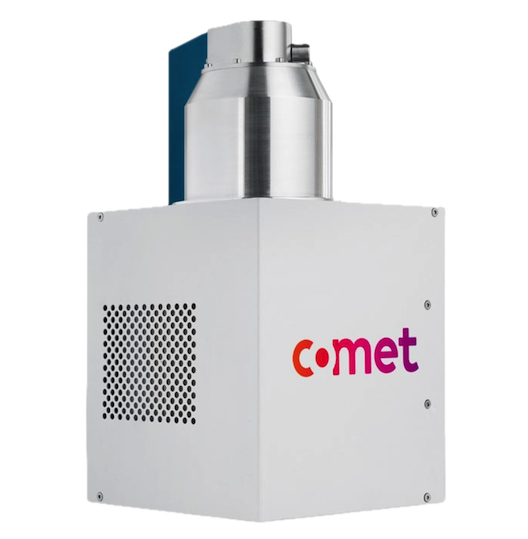
\includegraphics[width=\textwidth]{Microfocus.png}
        \caption{Produktdarstellung des Microfocus-Moduls}
        \label{fig:microfocus_product}
    \end{subfigure}
    
    \vspace{0.5cm}
    
    \begin{subfigure}{0.80\textwidth}
        \centering
        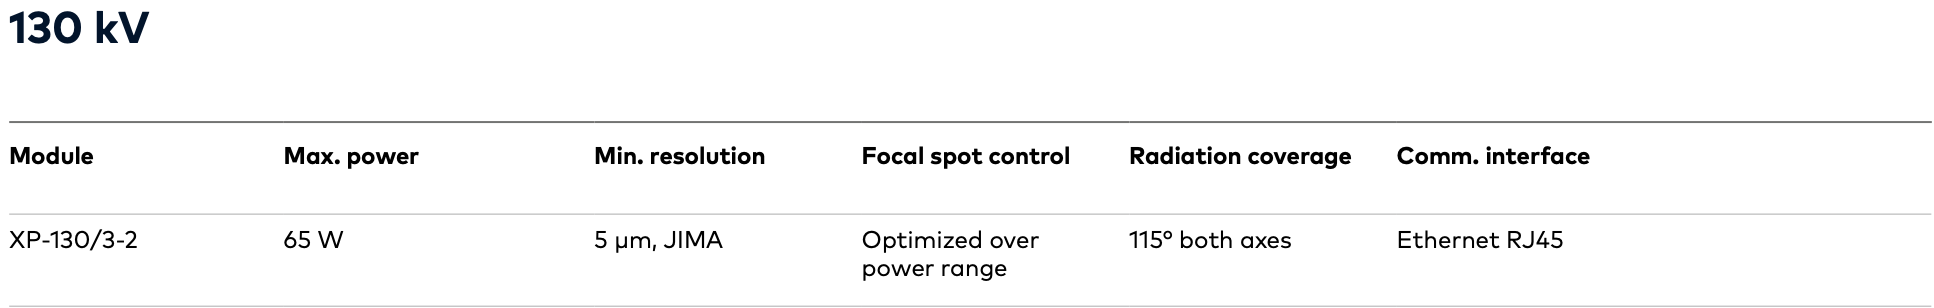
\includegraphics[width=\textwidth]{Microfocus-Specs.png}
        \caption{Technische Spezifikationen des Microfocus-Moduls}
        \label{fig:microfocus_specs}
    \end{subfigure}
    
    \caption{Microfocus-Modul und zugehörige Produktspezifikationen}
    \label{fig:microfocus_overview}
\end{figure}

\textbf{FXE Series} (nano focus) ist ein offenes Röntgenmodul für hochauflösende Prüf- und Messaufgaben, bei denen feinste Strukturen sichtbar gemacht werden müssen. Typische Anwendungen sind die zerstörungsfreie Qualitätskontrolle, Offline-Inspektion und die Vermessung sehr kleiner Defekte bis in den Submikrometerbereich.
Je nach Ausführung erreicht die FXE-Serie Auflösungen bis 0{,}5~µm und ist damit besonders für Anwendungen geeignet, bei denen maximale Detailerkennbarkeit im Vordergrund steht.
\\
\\
\begin{figure}[H]
    \centering
    
    \begin{subfigure}{0.40\textwidth}
        \centering
        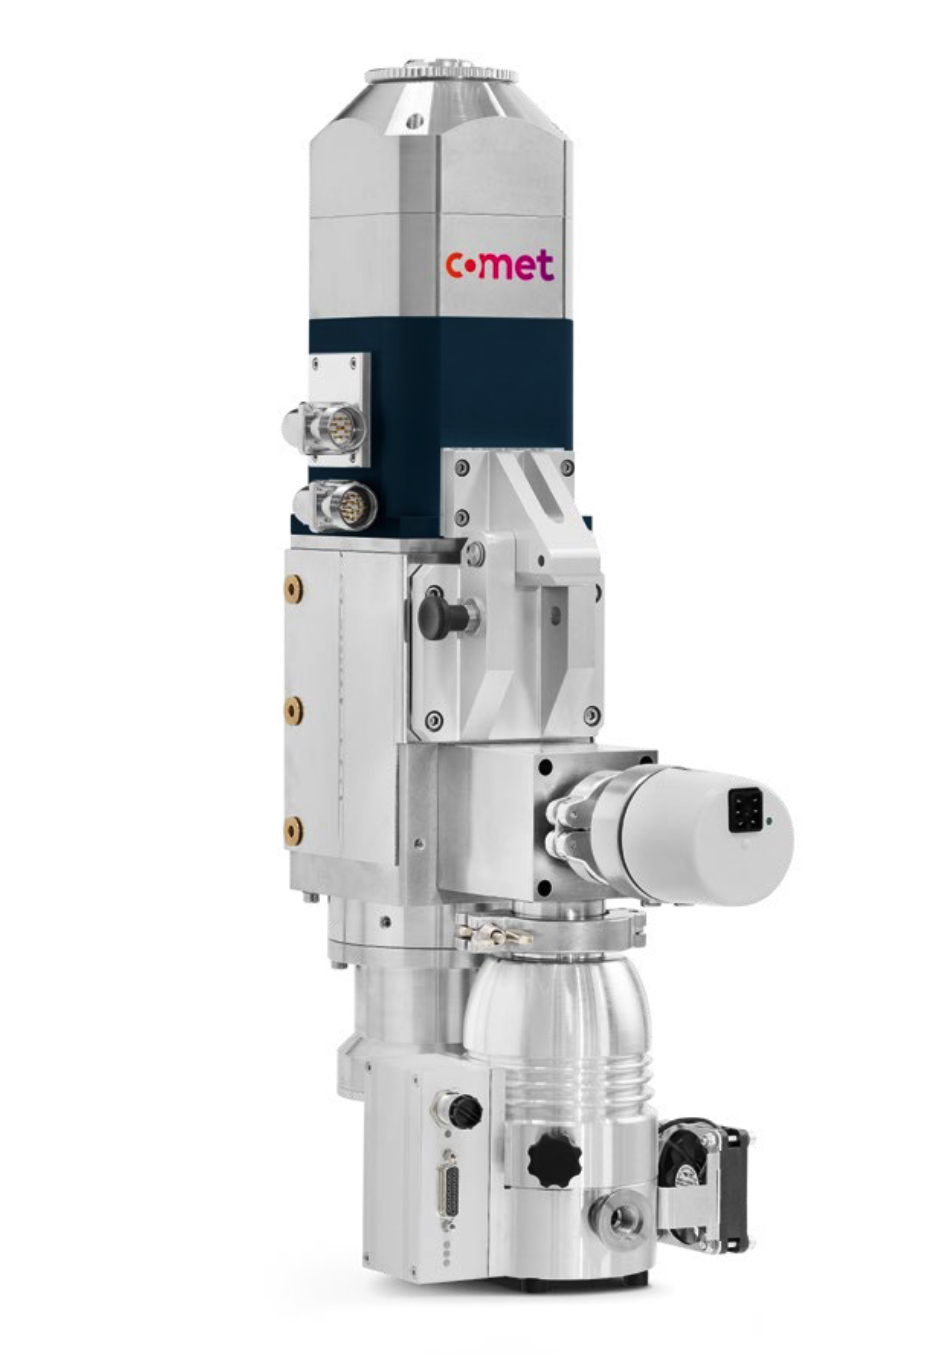
\includegraphics[width=\textwidth]{Nanofocus.png}
        \caption{Produktdarstellung des Nanofocus-Moduls}
        \label{fig:nanofocus_product}
    \end{subfigure}
    
    \vspace{0.5cm}
    
    \begin{subfigure}{0.80\textwidth}
        \centering
        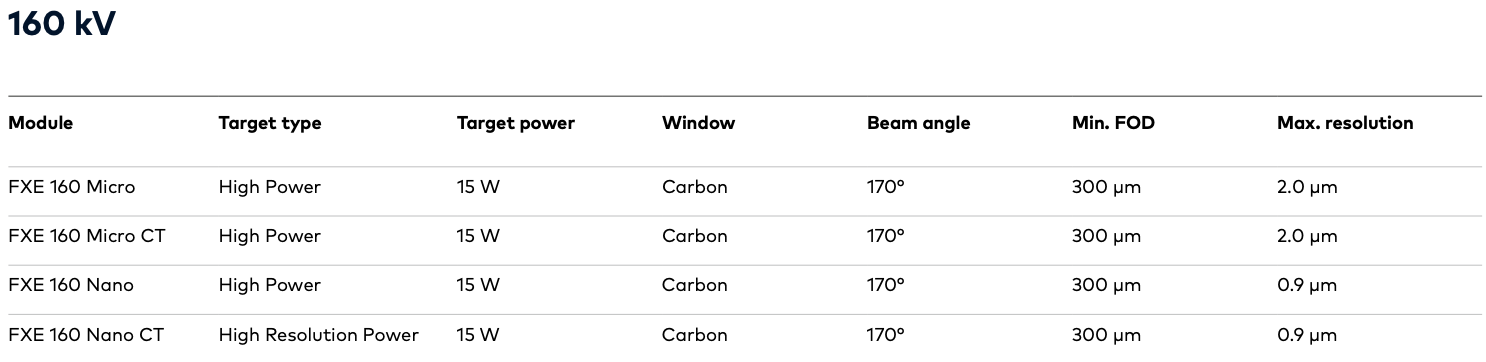
\includegraphics[width=\textwidth]{Nanofocus-Specs.png}
        \caption{Technische Spezifikationen des Nanofocus-Moduls}
        \label{fig:nanofocus_specs}
    \end{subfigure}
    
    \caption{Nanofocus-Modul und zugehörige Produktspezifikationen}
    \label{fig:nanofocus_overview}
\end{figure}


\textbf{iXRS MesoFocus Series} (meso focus) ist ein geschlossenes Röntgenmodul für die Inspektion größerer oder materialinhomogener Bauteile in industriellen Anwendungen. Typische Einsatzbereiche sind Batterien, additiv gefertigte Bauteile, Carbonfaserstrukturen und Gusskomponenten.
Die MesoFocus-Technologie ermöglicht die Erkennung von Strukturen bis etwa 25~µm und zeichnet sich durch eine hohe Stabilität aus, da der Fokuspunkt im Vergleich zu konventionellen Microfocus-Röhren nur gering durch thermische Änderungen beeinflusst wird.
\\

\begin{figure}[H]
    \centering
    
    \begin{subfigure}{0.40\textwidth}
        \centering
        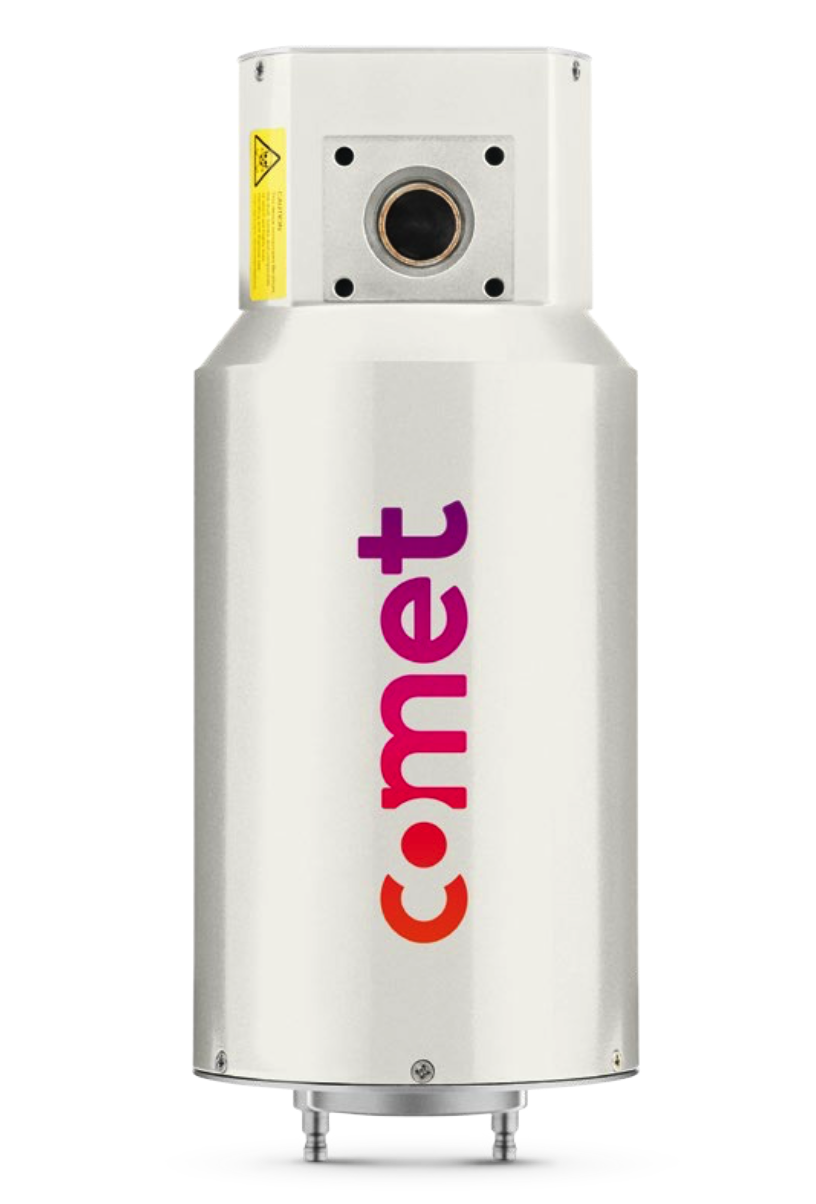
\includegraphics[width=\textwidth]{Mesofocus.png}
        \caption{Produktdarstellung des MesoFocus-Moduls}
        \label{fig:mesofocus_product}
    \end{subfigure}
    
    \vspace{0.5cm}
    
    \begin{subfigure}{0.80\textwidth}
        \centering
        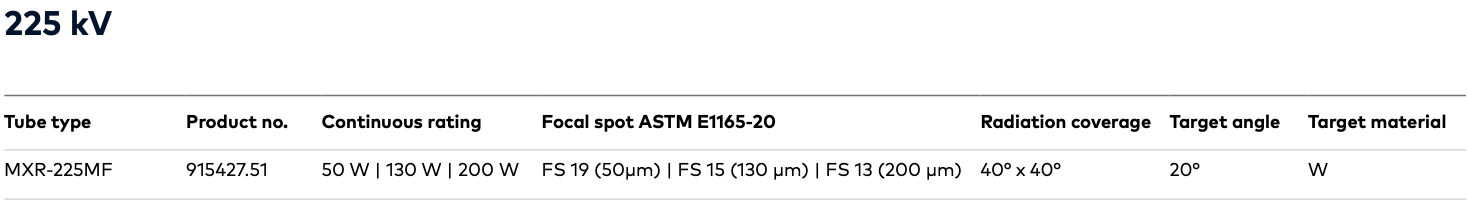
\includegraphics[width=\textwidth]{Mesofocus-Specs.png}
        \caption{Wesentliche technische Spezifikationen des MesoFocus-Moduls}
        \label{fig:mesofocus_specs}
    \end{subfigure}
    
    \caption{MesoFocus-Modul und zugehörige Produktspezifikationen}
    \label{fig:mesofocus_overview}
\end{figure}


\subsubsection{Einarbeitung in Team, Labor und Arbeitsumgebung}
Die ersten Tage wurden primär genutzt, um mir einen Einblick in das System zu geben. Nach der Übergabe der Arbeitswerkzeuge wurde ein Onboarding durchgeführt, um die Firmenstruktur zu erklären, mein Arbeitsbereich und Tätigkeitsfeld klar zu definieren und mir die Produkte im Labor vorzustellen. 
Mir wurde das Team, zuständig für die Testautomatisierung, vorgestellt, welches sich aus meinen 4 Kollegen zusammensetzt, welche alle in der Softwareentwicklung tätig sind mit Hintergrund in Elektrotechnik und Physik.
Im Labor wurde mir die Produktpalette vorgestellt, ihre Funktionen und Einsatzbereiche erklärt. Die Produkte teilten sich auf in ihren Tätigkeiten, ein Teil führte den Röntgentest auf einem Testobjekt aus, andere waren lediglich da, um die Stabilität für die Inputwerte zu testen und außerhalb vom Labor neben den Arbeitsplätzen waren Module, die Simulationen der Geräte durchführten. 
\\
\\

\subsection{Durchführung der Arbeiten}

\subsubsection{Analyse der bestehenden Testpipeline und Einarbeitung in die Werkzeuge}
Für den Xplorer waren bereits die meisten Tests in der Testpipeline integriert und auf dem Main Branch in der Umgebung Git implementiert. Jeden Abend und nach expliziten Abfragen wurden diese Tests ausgeführt und auf ihre Korrektheit geprüft.
Die Aufgabe bestand darin, diese Tests generisch zu gestalten, da sie davor für hardcodierte Werte ausgelegt waren. In dem vorliegenden Fall ging es erstmals nur um die Tests für die Maxima und Minima Inputs sowie Outputs. Die erste Woche wurde hauptsächlich genutzt, um sich mit der Umgebung vertraut zu machen, die Testabläufe zu verstehen und sich Gedanken zu machen über die technischen Grenzen des Systems.
Ich wurde in die Softwareentwicklungsprozesse und die dazugehörigen Werkzeuge eingeführt, dabei sollte ich eigenständig die zu aktualisierenden Tests anschauen und sie mit bereits generisch umgewandelten vergleichen und die Logik dahinter verstehen.
Die Arbeitsumgebung bestand aus verschiedener Software, die Entwicklung wurde mittels Python in der Softwareumgebung Visual Studio Code durchgeführt, Git für die Versionskontrolle und Speicherung von Veränderungen, Jenkins für die Testautomatisierung und die Testpipeline, Jira für die Projektplanung und Dokumentation der Aufgaben, Confluence für die Dokumentation der Testfälle und die Kommunikation mit den Kollegen.
\\
\\

\subsubsection{Parametrisierung und Implementierung von Grenzwerttests}
Ein Teil der Aufgabe bestand darin, die Werte, die festgesetzt wurden, mittels Variablen aus einer Produktdatenbank auszulesen und sie somit flexibel zu gestalten. Ein realer Fall war die Änderung von einem Grenzwert für die Röhrenspannung eines Produktes, aufgetragen von der Abteilung zuständig für die internen Komponenten.
Typische Tests waren die Überprüfung der Eingaben für die Spannung und des Emissionsstroms, die vorerst auf den Simulationen getestet wurden, um sicherzustellen, dass keine Arbeitspunkte außerhalb der Grenzen angefahren werden und diese immer auf die Grenzwerte gedrosselt oder hochgefahren werden.
Zur Beschreibung und Prüfung der relevanten Betriebsparameter der Röntgenmodule wurden mehrere grundlegende technische Zusammenhänge herangezogen. Die elektrische Röhrenleistung ergibt sich aus \(P = U \cdot I\), wobei bei Verwendung von \(\si{\kilo\volt}\) und \(\si{\milli\ampere}\) direkt \(P[\si{\watt}] = U[\si{\kilo\volt}] \cdot I[\si{\milli\ampere}]\) gilt.
Für die Parametervalidierung musste jeder gesetzte Sollwert innerhalb der produktspezifischen Grenzen liegen, also \(x_{\min} \leq x_{\mathrm{set}} \leq x_{\max}\). Zur Überprüfung des Grenzverhaltens wurden Testwerte gezielt knapp unterhalb bzw. oberhalb der Grenzen gewählt, beispielsweise \(x_{\mathrm{test,low}} = x_{\min}(1-\alpha)\) und \(x_{\mathrm{test,high}} = x_{\max}(1+\alpha)\) mit einer kleinen relativen Abweichung \(\alpha\), etwa \(5\,\%\).
Für den Vergleich zwischen Soll- und Istwert wurden der absolute Fehler \(e_{\mathrm{abs}} = |x_{\mathrm{actual}} - x_{\mathrm{set}}|\) und der relative Fehler \(e_{\mathrm{rel}} = \frac{|x_{\mathrm{actual}} - x_{\mathrm{set}}|}{x_{\mathrm{set}}}\) betrachtet.
Zusätzlich war für das Verhalten beim Hoch- und Herunterfahren von Spannung und Strom die Rampensteigung \(r = \frac{\Delta x}{\Delta t}\) relevant. Diese Zusammenhänge waren insbesondere für die Generisierung der Tests und die automatische Prüfung von Grenz- und Kombinationsfällen relevant, da die Comet-Generatoren für Spannung, Emissionsstrom, Rampenzeiten und Maximalleistung produktspezifische Grenzwerte vorgeben.
Zur Überprüfung werden Werte unterhalb und oberhalb der Grenzen angefahren, um das Verhalten des Systems zu überprüfen. Im Code müssen die betroffenen Komponenten mit den Werten gesetzt werden und nach einer gewissen Zeit, die in den Spezifikationen festgelegt wurde, abgefragt werden, um ihre Korrektheit zu überprüfen.

\subsubsection{Tests von Heater, Emission und Regelverhalten}
Eine weitere Abfrage bestand darin, die Werte des Heaters zu überprüfen, diese ist dafür zuständig, die Kathode zu erhitzen und bestimmt je nach Temperatur die Anzahl der in Bewegung gesetzten Elektronen. Die Ansteuerung hier ist relativ empfindlich, da die Zeit bis zum Erreichen und die des Haltens der Temperatur nur eine geringe Marge hat.
Bei Abweichungen differenzieren sich die Anzahl der Elektronen und oder kann es zu erhöhter Abreibung des Heizdrahtes kommen. Neben dem Testen der Zeit für das ramp up, steady state und cool off, ist weiterhin wichtig, die emission current zu überprüfen und sicherzustellen, dass sie intern korrekt geregelt wird. Es handelt sich hier um ein closed Loop System, welches für eine stabile Emission sorgt.
\\
\subsubsection{Beispiel eines automatisierten Emissionsgrenzwerttests}

\begin{lstlisting}[style=pythonwide, caption={Vereinfachtes Beispiel eines automatisierten Pytest-Grenzwerttests für Emissionslimits}, label={lst:emission_limits}]
import time
import pytest

@pytest.mark.parametrize("test_case", emission_limit_test_cases)
def test_emission_limits(system, test_case):
    # Initialen gueltigen Betriebszustand herstellen
    system.apply_setpoints(valid_setpoints)
    system.ramp_up_until_ready()

    # Testwert fuer den Emissionsgrenzbereich setzen
    system.set_emission_limit(test_case["limit_value"])

    # Kurz warten, bis der neue Zustand uebernommen wurde
    time.sleep(1)

    # Relevante Werte auslesen
    state = system.get_state()
    emission_setpoint = system.get_emission_setpoint()
    emission_applied = system.get_emission_applied()
    emission_actual = system.measure_emission()

    # Pruefen, ob sich das System im erwarteten Zustand befindet
    assert state["mode"] == "xray_on"
    assert state["status"] == "reached"

    # Pruefen, ob Soll-, angewendeter und gemessener Wert konsistent sind
    assert emission_setpoint == valid_setpoints["emission"]
    assert emission_applied == test_case["expected_value"]
    assert pytest.approx(
        emission_actual,
        abs=system.get_allowed_error("emission")
    ) == test_case["expected_value"]

    # Urspruenglichen Grenzwert zuruecksetzen
    system.set_emission_limit(default_emission_limit)
\end{lstlisting}

Listing~\ref{lst:emission_limits} zeigt schematisch den Aufbau eines automatisierten Tests zur Prüfung von Emissionsgrenzwerten.
Zunächst wird ein gültiger Ausgangszustand des Systems hergestellt, indem zulässige Setpoints gesetzt und das Modul kontrolliert hochgefahren wird.
Anschließend wird ein produktspezifischer Grenzwert für die Emission vorgegeben.
Nach einer kurzen Wartezeit werden sowohl der Betriebszustand als auch Soll-, angewendete und gemessene Emissionswerte ausgelesen.
Die anschließenden Prüfungen stellen sicher, dass das System den erwarteten Zustand erreicht hat und dass die tatsächlich übernommenen Werte innerhalb des zulässigen Toleranzbereichs liegen.
Besonders anzumerken, der folgende Code arbeitet lediglich mit ausglesenen Werten aus der Produkdatenbank, somit bleibt er für alle Produkte generisch und passt sich auch an veränderung der Datenbanken an.
\\

\subsubsection{Struktur der Testfälle und Kombination technischer Grenzwerte}
Häufig wurden für die Abfrage einzelner Parameter vier Testfälle erstellt, jeweils einen für das Über- und Unterschreiten der Grenzwerte um eine geringe Marge, wie 5\%, und jeweils ein Test, der auf die Konvergenz gegen Null und unendlich prüft. Es wurden auch Testfälle erstellt, welche die Kombination von Grenzwerten prüfen, wie zum Beispiel die Röhrenspannung und der Emissionsstrom, da diese in einem engen Zusammenhang stehen. 
Die Grenzwertabfragen konnten daher nicht für alle Produkte identisch übernommen werden. Ursache hierfür war, dass die zulässigen Betriebsbereiche produktspezifisch durch die Kombination aus Hochspannung, Emissionsstrom, maximaler Röhrenleistung und Fokuscharakteristik bestimmt wurden. Während bei einzelnen Produkten einfache feste Grenzwerte getestet werden konnten, mussten bei anderen Produkten gekoppelte Grenzen berücksichtigt werden, bei denen sich der zulässige Bereich eines Parameters in Abhängigkeit eines anderen Parameters veränderte.
Dies war insbesondere dann relevant, wenn dieselbe Produktfamilie in unterschiedlichen Leistungs- oder Fokusmodi betrieben werden konnte oder wenn die Stabilität des Focal Spots durch thermische oder stromabhängige Effekte beeinflusst wurde.
\\
\\

\subsubsection{Übertragung auf weitere Produkte und produktspezifische Unterschiede}
Nachdem für den Xplorer die meisten Tests angepasst wurden und sie generisch und nach dem DRY Prinzip gestaltet wurden, war der nächste Schritt die Anpassung der Tests für die anderen Produkte, welche teilweise noch nicht in der Testpipeline integriert waren.
Manche Tests ließen sich direkt übernehmen, da durch die generische Form lediglich die Parameter geändert wurden und die Syntax gleich blieb, andere mussten teilweise angepasst werden, da die Produkte sich in Komponenten und Funktionen unterschieden.
Ein wesentlicher Unterschied zwischen Nano Focus- und Meso Focus Röntgenquellen besteht in der Abhängigkeit der Focal-Spot Größe vom Emissionsstrom. Bei Nano Focus Röhren führt ein steigender Emissionsstrom aufgrund von Space-Charge Effekten zu einer deutlichen Vergrößerung des Elektronenstrahls und damit des Focal Spots.
Entsprechend müssen Testfälle die Beziehung zwischen Emissionsstrom und Spotgröße prüfen. Bei Meso Focus Röhren ist dieser Effekt deutlich geringer, weshalb hier eher thermische Stabilität und Leistungsstabilität über längere Betriebszeiten getestet werden.
Ein weiterer essenzieller Unterschied ist, dass das Warm-up Verhalten sich zwischen Nano Focus- und Meso Focus-Röntgenquellen deutlich unterscheidet. Bei Nano-Focus Systemen liegt der Schwerpunkt auf der Stabilisierung der Kathode und des Elektronenstrahls, da bereits geringe thermische Änderungen zu einer Veränderung des Focal Spots führen können. Entsprechend prüfen Testfälle die Stabilität der Spotgröße und der Emission.
Bei Meso-Focus Systemen steht hingegen die thermische Stabilisierung der Anode im Vordergrund, da diese mit deutlich höheren Leistungen betrieben werden. Warm-up Tests konzentrieren sich hier auf eine kontrollierte Leistungsrampe und die Überwachung thermischer Belastungen.
\\
\\

\subsubsection{Lokale Ausführung, Integration in die Pipeline und Zusammenarbeit im Team}
Alle der besprochenen Testfälle und noch einige weitere wurden selbstständig angepasst oder komplett neu erstellt. Die meisten wurden bereits vor Jahren implementiert, jedoch nie aktualisiert und teilweise sogar nie auf ihre Korrektheit überprüft. Mein Betreuer musste mir anfangs noch viel helfen, mich in der Programmierumgebung wohl zu fühlen und eigenständig zu arbeiten, jedoch wurde ich schnell selbständig und musste nur noch bei systembezogenen Fragen auf ihn zukommen.
Für mich wurden die drei Module als Simulationen bereitgestellt und nach erfolgreicher Einrichtung der Ansteuerung konnte ich meine Tests lokal laufen lassen. Nach Absprache mit meinem Betreuer konnte ich diese auch abends in die Testpipeline integrieren. Bei lokalen oder online Fehlmeldungen musste ich mich durch die Pytest-Logs lesen und aus den Errors meinen Fehler herausfinden und dementsprechend anpassen.
Für die Auswertung der real-time Simulationen stand mir ein Dashboard zur Verfügung, welches mein Betreuer programmiert hat und mir die Freiheit gab, es nach meinen Bedürfnissen anzupassen. Es zeigte mir die Zustände einzelner Komponenten an, ob diese in ihre Limits geraten sind. Außerdem wurden die gesetzten und angefahrenen Setpoints visuell angezeigt.
Nach mehrfacher korrekter Ausführung in der Pipeline und Abschluss einzelner Themenblöcke konnte ich zusammen mit meinem Betreuer meinen Git-Branch auf den Main Branch pushen und somit meine Arbeit offiziell ins System integrieren.
\\
\\

In den täglich und wöchentlich angesetzten Meetings mit meinem Team und mit der ganzen Abteilung wurden wir gegenseitig über den aktuellen Fortschritt auf dem Laufenden gehalten, wie auch ich über meinen Fortschritt informiert habe.
Teilweise habe ich auch anderen Kollegen geholfen, wie bei der Suche nach Problemstellen, oder bei der Recherche gewisser Themen, um zuvor nicht behandelte Testfälle abzufragen. 

\subsection{Ergebnisse und Einordnung}
\hl{Testergebnisse, was nach mir alles automatisch in der Pipeline läuft.
Das Testoverlay nachprogrammieren und vorstellen, eventuell Video erstellen.
Verständnis der Produkte.}

\hl{Zu Überprüfen:
\\
\\
Reihenfolge des Textes
\\
\\
Zusammenhang des Systems - Generator zu Modul - etc.
\\
\\
Darstellung zeigen und Prozess erklären der Röntgenstrahlung. Alles selber nachbauen!!
\\
\\
}
\newpage

\section{Praktikumsstelle II: PricewaterhouseCoopers GmbH}
\subsection{Lorem Ipsum}
\subsection{Lorem Ipsum}
\subsection{Summarium}

\newpage

\newpage

\section{Einheits-/ Formelverzeichnis}

% Literaturverzeichnis
\section{Literaturverzeichnis}
\begin{thebibliography}{99}
    \bibitem{quelle1} Autor Vorname Nachname, \textit{Titel des Buches}, Verlag, Jahr.
    \bibitem{quelle2} Autor Vorname Nachname, \textit{Titel des Artikels}, Zeitschrift, Jahr.
    \bibitem{quelle3} Autor Vorname Nachname, \textit{Titel der Webseite}, URL: \url{https://example.com}, Zugriff am: 5. März 2026.
\end{thebibliography}

\end{document}